% One cluster's datapath (itmn_m2/src/mamba/M_Cluster.v, Reduce16Wide.v and the fabric rows of Mamba_Cluster.v).
\documentclass[tikz,border=4pt]{standalone}
% Shared style of the RTL diagrams. Build one with: tectonic fig_x.tex
\usepackage{tikz}
\usetikzlibrary{arrows.meta,positioning,fit,calc,backgrounds,shapes.geometric}
\usepackage[T1]{fontenc}
\usepackage{lmodern}
% opaque background, so the SVGs stay readable on dark pages
\tikzset{every picture/.append style={show background rectangle,
         background rectangle/.style={fill=white, draw=none}, inner frame sep=2pt}}
\definecolor{inkA}{HTML}{0B0B0B}
\definecolor{inkB}{HTML}{52514E}
\definecolor{rule}{HTML}{C3C2B7}
\definecolor{fillA}{HTML}{F0EFEC}
\definecolor{fillPE}{HTML}{CDE2FB}
\definecolor{fillRow}{HTML}{FBE0D3}
\definecolor{fillMem}{HTML}{E5F4EC}
\definecolor{fillCtl}{HTML}{FDF0C8}
\definecolor{fillReg}{HTML}{F6C9A8}
\definecolor{ctlink}{HTML}{8A6A00}
\tikzset{
  blk/.style={draw=inkB, line width=0.5pt, rounded corners=1.5pt, align=center, font=\scriptsize, inner sep=2pt},
  pe/.style={blk, fill=fillPE},
  row/.style={blk, fill=fillRow},
  mem/.style={blk, fill=fillMem},
  ctl/.style={blk, fill=fillCtl},
  plain/.style={blk, fill=white},
  grp/.style={draw=rule, line width=0.6pt, rounded corners=3pt, inner sep=4pt},
  dgrp/.style={draw=inkB, dashed, line width=0.5pt, rounded corners=3pt, inner sep=4pt},
  arr/.style={-{Stealth[length=3pt]}, line width=0.5pt, draw=inkB},
  darr/.style={{Stealth[length=3pt]}-{Stealth[length=3pt]}, line width=0.5pt, draw=inkB},
  carr/.style={-{Stealth[length=2.5pt]}, line width=0.4pt, draw=ctlink, densely dashed},
  lbl/.style={font=\scriptsize, text=inkB, align=center},
  tlbl/.style={font=\tiny, text=inkB, align=center},
  clbl/.style={font=\tiny, text=ctlink, align=center},
  opc/.style={circle, draw=inkB, fill=white, line width=0.5pt, minimum size=0.42cm, inner sep=0pt, font=\scriptsize},
  mux/.style={trapezium, trapezium stretches=true, trapezium angle=70, draw=inkB, fill=fillA, line width=0.5pt, minimum height=0.38cm,
              inner sep=1pt, font=\tiny, shape border rotate=180},
  regbar/.style={draw=inkB, fill=fillReg, line width=0.5pt, minimum height=0.16cm, inner sep=0pt},
}
% bus width mark: \bw{coordinate}{width}
\newcommand{\bw}[2]{\draw[line width=0.4pt, draw=inkB] ($(#1)+(-0.06,-0.06)$) -- ($(#1)+(0.06,0.06)$)
  node[tlbl, anchor=west, inner sep=1pt] {#2};}

\begin{document}
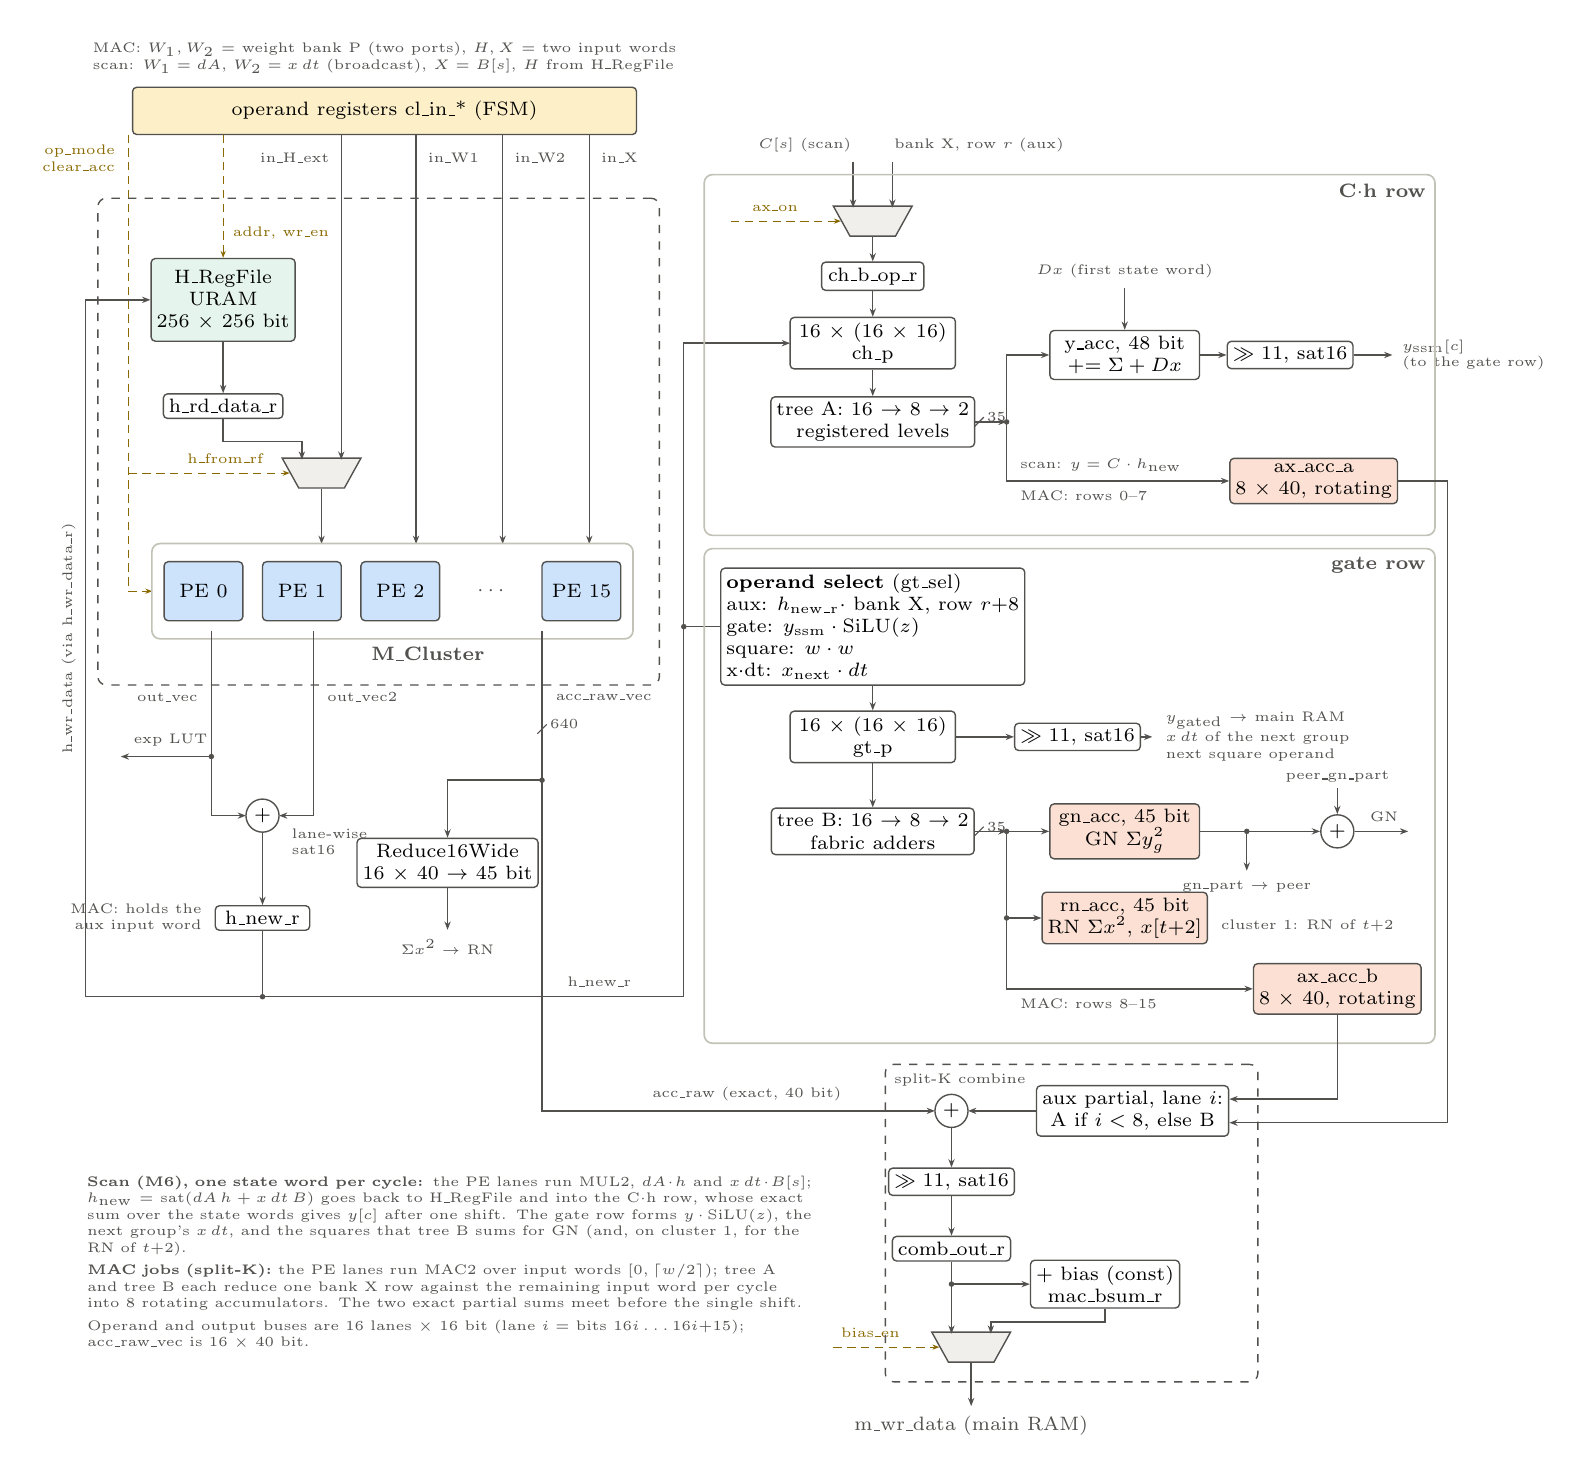
\begin{tikzpicture}[x=1cm,y=1cm]
  % ================================================================ operand registers (set by the FSM)
  \node[ctl, minimum width=6.4cm, minimum height=0.6cm] (opr) at (3.8,13.7) {operand registers cl\_in\_* (FSM)};
  \node[tlbl, anchor=south, align=left] at (3.8,14.05) {%
    MAC: $W_1, W_2$ = weight bank P (two ports), $H, X$ = two input words\\
    scan: $W_1 = dA$, $W_2 = x\,dt$ (broadcast), $X = B[s]$, $H$ from H\_RegFile};

  % ================================================================ M_Cluster
  % state RAM
  \node[mem, minimum width=1.6cm, minimum height=1.05cm] (hrf) at (1.75,11.3) {H\_RegFile\\URAM\\256 $\times$ 256 bit};
  \draw[carr] (1.75,13.4) -- (hrf.north) node[clbl, pos=0.8, right] {addr, wr\_en};
  \node[plain, minimum width=1.3cm] (hrr) at (1.75,9.95) {h\_rd\_data\_r};
  \draw[arr] (hrf.south) -- (hrr.north);
  \node[mux, minimum width=1.0cm] (hmx) at (3.0,9.1) {};
  \draw[arr] (hrr.south) -- (1.75,9.5) -| (2.75,9.27);
  \draw[arr] (3.25,13.4) -- (3.25,9.27);
  \node[tlbl, anchor=east] at (3.22,13.1) {in\_H\_ext};
  \draw[carr] (0.55,9.1) -- (hmx.west) node[clbl, pos=0.6, above] {h\_from\_rf};
  \draw[arr] (hmx.south) -- (3.0,8.2);
  % other operands
  \foreach \n/\x in {in\_W1/4.2, in\_W2/5.3, in\_X/6.4} {
    \draw[arr] (\x,13.4) -- (\x,8.2);
    \node[tlbl, anchor=west] at (\x+0.03,13.1) {\n};}
  \draw[carr] (0.55,13.4) -- (0.55,7.6) -- (0.85,7.6);
  \node[clbl, anchor=east, align=right] at (0.5,13.1) {op\_mode\\clear\_acc};
  % PE lanes
  \foreach \n/\x in {PE 0/1.5, PE 1/2.75, PE 2/4.0, PE 15/6.3} {\node[pe, minimum width=1.0cm, minimum height=0.75cm] at (\x,7.6) {\n};}
  \node[lbl] at (5.15,7.6) {$\cdots$};
  \node[grp, fit={(0.95,8.1) (6.85,7.1)}, inner sep=3pt] (pea) {};
  \node[dgrp, fit={(0.3,12.45) (7.15,6.55)}] (mcl) {};
  \node[lbl] at (4.35,6.8) {\textbf{M\_Cluster}};

  % ================================================================ PE outputs
  \draw[arr] (1.6,7.1) -- (1.6,4.75) -- ($(1.6,4.75)+(0.44,0)$);
  \draw[arr] (2.9,7.1) -- (2.9,4.75) -- ($(2.9,4.75)+(-0.44,0)$);
  \draw[arr] (5.8,7.1) -- (5.8,1.0) -- (10.79,1.0);
  \node[tlbl, anchor=east] at (1.55,6.25) {out\_vec};
  \node[tlbl, anchor=west] at (2.95,6.25) {out\_vec2};
  \node[tlbl, anchor=west] at (5.85,6.25) {acc\_raw\_vec};
  \bw{5.8,5.85}{640}
  % exp LUT
  \draw[arr] (1.6,5.5) -- (0.45,5.5) node[tlbl, anchor=south, pos=0.45] {exp LUT};
  % h_new = sat(dA h + x dt B)
  \node[opc] (hadd) at (2.25,4.75) {$+$};
  \node[tlbl, anchor=west, align=left] at (2.5,4.42) {lane-wise\\sat16};
  \node[plain, minimum width=1.2cm] (hnr) at (2.25,3.45) {h\_new\_r};
  \draw[arr] (hadd.south) -- (hnr.north);
  \node[tlbl, anchor=east, align=right] at (1.6,3.45) {MAC: holds the\\aux input word};
  \draw[arr] (hnr.south) -- (2.25,2.45) -- (0.0,2.45) -- (0.0,11.3) -- (hrf.west);
  \node[tlbl, anchor=south, rotate=90] at (0.0,7.0) {h\_wr\_data (via h\_wr\_data\_r)};
  \draw[arr] (2.25,2.45) -- (7.6,2.45) -- (7.6,10.75) -- (8.95,10.75);
  \draw[arr] (7.6,7.15) -- ($(7.6,7.15)+(0.75,0)$);
  \fill[inkB] (2.25,2.45) circle (0.035) (7.6,7.15) circle (0.035) (1.6,5.5) circle (0.035) (5.8,5.2) circle (0.035);
  \node[tlbl, anchor=south west] at (6.0,2.45) {h\_new\_r};
  % Reduce16Wide
  \node[plain, minimum width=1.6cm] (rw) at (4.6,4.15) {Reduce16Wide\\16 $\times$ 40 $\to$ 45 bit};
  \draw[arr] (5.8,5.2) -| (rw.north);
  \draw[arr] (rw.south) -- (4.6,3.3) node[tlbl, anchor=north] {$\Sigma x^2 \to$ RN};

  % ================================================================ C*h row (tree A)
  \node[mux, minimum width=1.0cm] (chmx) at (10.0,12.3) {};
  \draw[arr] (9.75,13.05) -- (9.75,12.47);
  \draw[arr] (10.25,13.05) -- (10.25,12.47);
  \node[tlbl, anchor=south east] at (9.85,13.05) {$C[s]$ (scan)};
  \node[tlbl, anchor=south west] at (10.15,13.05) {bank X, row $r$ (aux)};
  \draw[carr] (8.2,12.3) -- (chmx.west) node[clbl, pos=0.4, above] {ax\_on};
  \node[plain, minimum width=1.3cm] (chb) at (10.0,11.6) {ch\_b\_op\_r};
  \draw[arr] (chmx.south) -- (chb.north);
  \node[plain, minimum width=2.1cm] (mula) at (10.0,10.75) {16 $\times$ (16 $\times$ 16)\\ch\_p};
  \draw[arr] (chb.south) -- (mula.north);
  \node[plain, minimum width=2.1cm] (tra) at (10.0,9.75) {tree A: 16 $\to$ 8 $\to$ 2\\registered levels};
  \draw[arr] (mula.south) -- (tra.north);
  \draw[arr] (tra.east) -- (11.7,9.75);
  \node[plain, minimum width=1.9cm] (yacc) at (13.2,10.6) {y\_acc, 48 bit\\$\mathrel{+}= \Sigma + D x$};
  \node[plain, minimum width=1.4cm] (ysat) at (15.3,10.6) {$\gg 11$, sat16};
  \node[tlbl, anchor=south] (dx) at (13.2,11.45) {$D x$ (first state word)};
  \draw[arr] (dx.south) -- (yacc.north);
  \draw[arr] (11.7,9.75) |- (yacc.west);
  \draw[arr] (yacc.east) -- (ysat.west);
  \draw[arr] (ysat.east) -- (16.6,10.6) node[tlbl, anchor=west, align=left] {$y_\mathrm{ssm}[c]$\\(to the gate row)};
  \node[row, minimum width=1.6cm] (axa) at (15.6,9.0) {ax\_acc\_a\\8 $\times$ 40, rotating};
  \draw[arr] (11.7,9.75) |- (axa.west);
  \fill[inkB] (11.7,9.75) circle (0.035);
  \node[tlbl, anchor=south west] at (11.75,9.0) {scan: $y = C \cdot h_\mathrm{new}$};
  \node[tlbl, anchor=north west] at (11.75,9.0) {MAC: rows 0--7};
  \bw{11.35,9.75}{35}
  \node[grp, fit={(8.0,12.75) (17.0,8.45)}] (rowa) {};
  \node[lbl, anchor=north east] at (rowa.north east) {\textbf{C$\cdot$h row}};

  % ================================================================ gate row (tree B)
  \node[plain, align=left] (gsel) at (10.0,7.15) {%
    \textbf{operand select} (gt\_sel)\\
    aux: $h_\mathrm{new\_r} \cdot$ bank X, row $r{+}8$\\
    gate: $y_\mathrm{ssm} \cdot \mathrm{SiLU}(z)$\\
    square: $w \cdot w$\\
    x$\cdot$dt: $x_\mathrm{next} \cdot dt$};
  \node[plain, minimum width=2.1cm] (mulb) at (10.0,5.75) {16 $\times$ (16 $\times$ 16)\\gt\_p};
  \draw[arr] (gsel.south) -- (mulb.north);
  \node[plain, minimum width=1.4cm] (gsat) at (12.6,5.75) {$\gg 11$, sat16};
  \draw[arr] (mulb.east) -- (gsat.west);
  \draw[arr] (gsat.east) -- (13.55,5.75);
  \node[tlbl, anchor=west, align=left] at (13.6,5.75) {$y_\mathrm{gated}$ $\to$ main RAM\\$x\,dt$ of the next group\\next square operand};
  \node[plain, minimum width=2.1cm] (trb) at (10.0,4.55) {tree B: 16 $\to$ 8 $\to$ 2\\fabric adders};
  \draw[arr] (mulb.south) -- (trb.north);
  \draw[arr] (trb.east) -- (11.7,4.55);
  \node[row, minimum width=1.9cm] (gna) at (13.2,4.55) {gn\_acc, 45 bit\\GN $\Sigma y_g^2$};
  \node[row, minimum width=1.9cm] (rna) at (13.2,3.45) {rn\_acc, 45 bit\\RN $\Sigma x^2$, $x[t{+}2]$};
  \node[row, minimum width=1.6cm] (axb) at (15.9,2.55) {ax\_acc\_b\\8 $\times$ 40, rotating};
  \draw[arr] (11.7,4.55) -- (gna.west);
  \draw[arr] (11.7,4.55) |- (rna.west);
  \draw[arr] (11.7,4.55) |- (axb.west);
  \fill[inkB] (11.7,4.55) circle (0.035) (11.7,3.45) circle (0.035);
  \node[tlbl, anchor=north west] at (11.75,2.55) {MAC: rows 8--15};
  \node[tlbl, anchor=west] at (14.3,3.35) {cluster 1: RN of $t{+}2$};
  % GN partial exchange
  \node[opc] (gns) at (15.9,4.55) {$+$};
  \draw[arr] (gna.east) -- (gns.west);
  \draw[arr] (14.75,4.55) -- (14.75,4.05) node[tlbl, anchor=north] {gn\_part $\to$ peer};
  \node[tlbl, anchor=south] at (15.9,5.05) {peer\_gn\_part};
  \draw[arr] (15.9,5.1) -- (gns.north);
  \draw[arr] (gns.east) -- (16.8,4.55) node[tlbl, anchor=south, pos=0.55] {GN};
  \fill[inkB] (14.75,4.55) circle (0.035);
  \bw{11.35,4.55}{35}
  \node[grp, fit={(8.0,8.0) (17.0,2.0)}] (rowb) {};
  \node[lbl, anchor=north east] at (rowb.north east) {\textbf{gate row}};

  % ================================================================ split-K combine
  \node[plain] (aux) at (13.3,1.0) {aux partial, lane $i$:\\A if $i < 8$, else B};
  \draw[arr] (axb.south) |- ($(aux.east)+(0,0.15)$);
  \draw[arr] (axa.east) -- (17.3,9.0) |- ($(aux.east)+(0,-0.15)$);
  \draw[arr] (aux.west) -- (11.21,1.0);
  \node[opc] (cadd) at (11.0,1.0) {$+$};
  \node[tlbl, anchor=south] at (8.4,1.0) {acc\_raw (exact, 40 bit)};
  \node[plain, minimum width=1.4cm] (csh) at (11.0,0.1) {$\gg 11$, sat16};
  \draw[arr] (cadd.south) -- (csh.north);
  \node[plain, minimum width=1.4cm] (cor) at (11.0,-0.75) {comb\_out\_r};
  \draw[arr] (csh.south) -- (cor.north);
  \node[plain, minimum width=1.5cm] (bias) at (12.95,-1.2) {+ bias (const)\\mac\_bsum\_r};
  \draw[arr] (cor.south) -- (11.0,-1.2) -- (bias.west);
  \node[mux, minimum width=1.0cm] (bmx) at (11.25,-2.0) {};
  \draw[arr] (11.0,-1.2) -- (11.0,-1.83);
  \draw[arr] (bias.south) |- (11.5,-1.68) -- (11.5,-1.83);
  \fill[inkB] (11.0,-1.2) circle (0.035);
  \draw[carr] (9.5,-2.0) -- (bmx.west) node[clbl, pos=0.35, above] {bias\_en};
  \draw[arr] (bmx.south) -- (11.25,-2.75) node[lbl, anchor=north] {m\_wr\_data (main RAM)};
  \node[dgrp, fit={(10.3,1.45) (14.75,-2.3)}] (cmb) {};
  \node[tlbl, anchor=north west] at (cmb.north west) {split-K combine};

  % ================================================================ notes
  \node[tlbl, anchor=north west, align=left, text width=9.2cm] at (-0.1,0.3) {%
    \textbf{Scan (M6), one state word per cycle:} the PE lanes run MUL2, $dA \cdot h$ and $x\,dt \cdot B[s]$;
    $h_\mathrm{new} = \mathrm{sat}(dA\,h + x\,dt\,B)$ goes back to H\_RegFile and into the C$\cdot$h row, whose
    exact sum over the state words gives $y[c]$ after one shift. The gate row forms $y \cdot \mathrm{SiLU}(z)$,
    the next group's $x\,dt$, and the squares that tree B sums for GN (and, on cluster 1, for the RN of
    $t{+}2$).\\[2pt]
    \textbf{MAC jobs (split-K):} the PE lanes run MAC2 over input words $[0, \lceil w/2 \rceil)$; tree A and
    tree B each reduce one bank X row against the remaining input word per cycle into 8 rotating accumulators.
    The two exact partial sums meet before the single shift.\\[2pt]
    Operand and output buses are 16 lanes $\times$ 16 bit (lane $i$ = bits $16i \ldots 16i{+}15$);
    acc\_raw\_vec is 16 $\times$ 40 bit.};
\end{tikzpicture}
\end{document}
